\documentclass[compress]{beamer}
\usepackage{graphicx,amsmath,amsthm,verbatim,bm}
\usepackage{longtable}
\usepackage{booktabs}       % professional-quality tables
\usepackage{tabularx}
\usepackage{multirow}
%\usetheme{Copenhagen}
%\useoutertheme[{options}]{tree}
%\setbeamertemplate{footline}[page number]
%\useoutertheme{infolines}
%\setbeamertem plate{headlirne}{}
%\useinnertheme{circles}
\usepackage{comment}
\setbeamertemplate{footline}[frame number]
%\usepackage{times}
%\usepackage[tbtags]{amsmath}
%\usepackage{amssymb}
\usepackage{amsfonts}
\usepackage{multirow}
%\usepackage{slfortheorems}
\usepackage{epsfig}
\usepackage{graphicx}
%\usepackage[small]{caption}
\usepackage[square]{natbib}
%\newcommand{\newblock}{}
\bibpunct{(}{)}{;}{a}{}{,}
\bibliographystyle{ims}
%\usepackage[letterpaper]{geometry}
\usepackage{color}
\setlength{\parindent}{0pt}
\usepackage{bbding}
\usepackage{longtable, booktabs}
\usepackage{amsfonts}
\usepackage{lipsum}
\usepackage{tikz} 
\usetikzlibrary{arrows, snakes, backgrounds, patterns, matrix, shapes, fit, 
calc, shadows, plotmarks}
\useinnertheme{circles}
\usepackage{tabularx}

\def\spacingset#1{\renewcommand{\baselinestretch}%
  {#1}\small\normalsize} \spacingset{1}
  
  \newcommand{\dblink}{\texttt{\upshape \lowercase{d-blink}}} % Name of scalable Bayesian ER model

\newcommand{\clusters}{\bm{\kappa}}
\newcommand{\cluster}[1]{\kappa_{#1}}
\newcommand{\sizes}{\bm{\mu}}
\newcommand{\size}[1]{\mu_{#1}}

\newcommand{\edist}{\bm{\gamma}}
\newcommand{\shape}{\eta}
\newcommand{\rate}{s}
\newcommand{\betaA}{u}
\newcommand{\betaB}{v}



\usepackage{tkz-berge}
\usetikzlibrary{fit,shapes}

\usepackage{calc}
\usetikzlibrary{decorations.markings}

\tikzstyle{vertex}=[circle, draw, inner sep=0pt, minimum size=6pt]
\newcommand{\vertex}{\node[vertex]}
\newcounter{Angle}


\usepackage{tabularx}

\let\oldvec\vec
\let\oldcomment\comment
\renewcommand{\comment}[1]{\textcolor{blue}{[#1]}}
\renewcommand\vec{\bm}
\newcommand{\simfn}{\texttt{sim}} % similarity function
\newcommand{\truncsimfn}{\underline{\simfn}} % truncated similarity function
\newcommand{\partfn}{\texttt{PartFn}} % partition function
\newcommand{\distfn}{\texttt{dist}} % distance function
\newcommand{\valset}{\mathcal{V}} % attribute value set
\newcommand{\entset}{\mathcal{E}} % set of records that make up an entity
\newcommand{\partset}{\mathcal{P}} % set of entities that make up a partition
\newcommand{\1}[1]{\mathbb{I}\!\left[#1\right]} % indicator function
\newcommand{\euler}{\mathrm{e}} % Euler's constant
\newcommand{\eber}{\texttt{EBER}} % Name of Bayesian ER model
\newcommand{\secref}[1]{\S\ref{#1}} % Section reference



\usepackage{listings}
\usepackage[ruled,lined]{algorithm2e}
\def\algorithmautorefname{Algorithm}
\SetKwIF{If}{ElseIf}{Else}{if}{then}{else if}{else}{endif}

\usepackage{longtable}



\theoremstyle{plain}
\usepackage{amsfonts}
\usepackage{epsfig}
\usepackage{graphicx}
%\usepackage[small]{caption}

\usepackage{zref-savepos}

\newcounter{restofframe}
\newsavebox{\restofframebox}
\newlength{\mylowermargin}
\setlength{\mylowermargin}{2pt}

\newenvironment{restofframe}{%
    \par%\centering
    \stepcounter{restofframe}%
    \zsavepos{restofframe-\arabic{restofframe}-begin}%
    \begin{lrbox}{\restofframebox}%
}{%
    \end{lrbox}%
    \setkeys{Gin}{keepaspectratio}%
    \raisebox{\dimexpr-\height+\ht\strutbox\relax}[0pt][0pt]{%
    \resizebox*{!}{\dimexpr\zposy{restofframe-\arabic{restofframe}-begin}sp-\zposy{restofframe-\arabic{restofframe}-end}sp-\mylowermargin\relax}%
        {\usebox{\restofframebox}}%
    }%
    \vskip0pt plus 1filll\relax
    \mbox{\zsavepos{restofframe-\arabic{restofframe}-end}}%
    \par
}


\usepackage{tikz}
\usetikzlibrary{arrows}

%\usepackage[usenames,dvipsnames]{xcolor}
\usepackage{tkz-berge}
\usetikzlibrary{fit,shapes}

\usepackage{calc}
\usetikzlibrary{decorations.markings}
%
%\tikzstyle{vertex}=[circle, draw, inner sep=0pt, minimum size=6pt]
%\newcommand{\vertex}{\node[vertex]}
%\newcounter{Angle}



%%%to add in new counter for slides in beamer
\newcommand{\beginbackup}{
   \newcounter{framenumbervorappendix}
   \setcounter{framenumbervorappendix}{\value{framenumber}}
}
\newcommand{\backupend}{
   \addtocounter{framenumbervorappendix}{-\value{framenumber}}
   \addtocounter{framenumber}{\value{framenumbervorappendix}} 
}


\newcommand*\oldmacro{}
\let\oldmacro\insertshortauthor
\renewcommand*\insertshortauthor{
  \leftskip=.3cm
\insertframenumber\,/\,\inserttotalframenumber\hfill\oldmacro}




\excludecomment{notbeamer}
\includecomment{beamer}

\newcommand{\lam}{\mathbf{\Lambda}}	
\newcommand{\bX}{\mathbf{X}}
\newcommand{\bY}{\mathbf{Y}}

\title[(Almost) All of Entity Resolution]
{(Almost) All of Entity Resolution}
\author[Rebecca C. Steorts, beka@stat.duke.edu]{Rebecca C. Steorts\\joint work with \textbf{Olivier Binette}, PhD Student, Department of Statistical Science Duke University} 

\institute{\normalsize Department of Statistical Science, affiliated faculty in Computer Science, Biostatistics and Bioinformatics, the information initiative at Duke (iiD) and \\the Social Science Research Institute (SSRI) \\ Duke University and U.S. Census Bureau\\ \vspace*{1em}

This work is supported by NSF CAREER Award 1652431 and the Alfred Sloan Foundation (DRB \#: CBDRB-FY20-309).

%\begin{figure}[htbp]
%\begin{center}
%\includegraphics{pics/banner}
%%\caption{default}
%\label{default}
%\end{center}
%\end{figure}
}
%\date{August 13, 2019}




\begin{document}
\begin{frame}
\titlepage
\end{frame}

%\frame{
%
%remark to self: merge in OB's nice introduction. 
%
%}

%\begin{frame}
%
%\begin{enumerate}
%\item Why record linkage?
%\item Terminology
%\item Challenges
%\item Pipeline approach 
%\item Deterministic record linkage 
%\item Probabilistic record linkage
%\item Modern  Probabilistic record linkage
%\item Clustering entity resolution
%\item Life after entity resolution 
%\item Open research questions
%\end{enumerate}
%\end{frame}





\frame{
\center
\Large

Entity resolution (record linkage or de-duplication) is the process of removing duplicated information from large noisy databases. 

\pause

\vspace*{1em}
The purpose of this review is to introduce one to the fundamentals of entity resolution, its applications, and modern developments over the past 61+ years. 

}

\frame{
\center
\Large

What is the purpose of entity resolution? 

}

%\frame{
%
%\begin{enumerate}
%\item Enumeration of individuals in census
%\item Enumeration of individuals in human rights conflict
%\item Understanding the analysis of co-authorship networks 
%\item Providing unique identifiers to voter records
%
%\textcolor{red}{Find better pictures of these}
%
%\end{enumerate}

\frame{

\begin{figure}[htbp]
\begin{center}
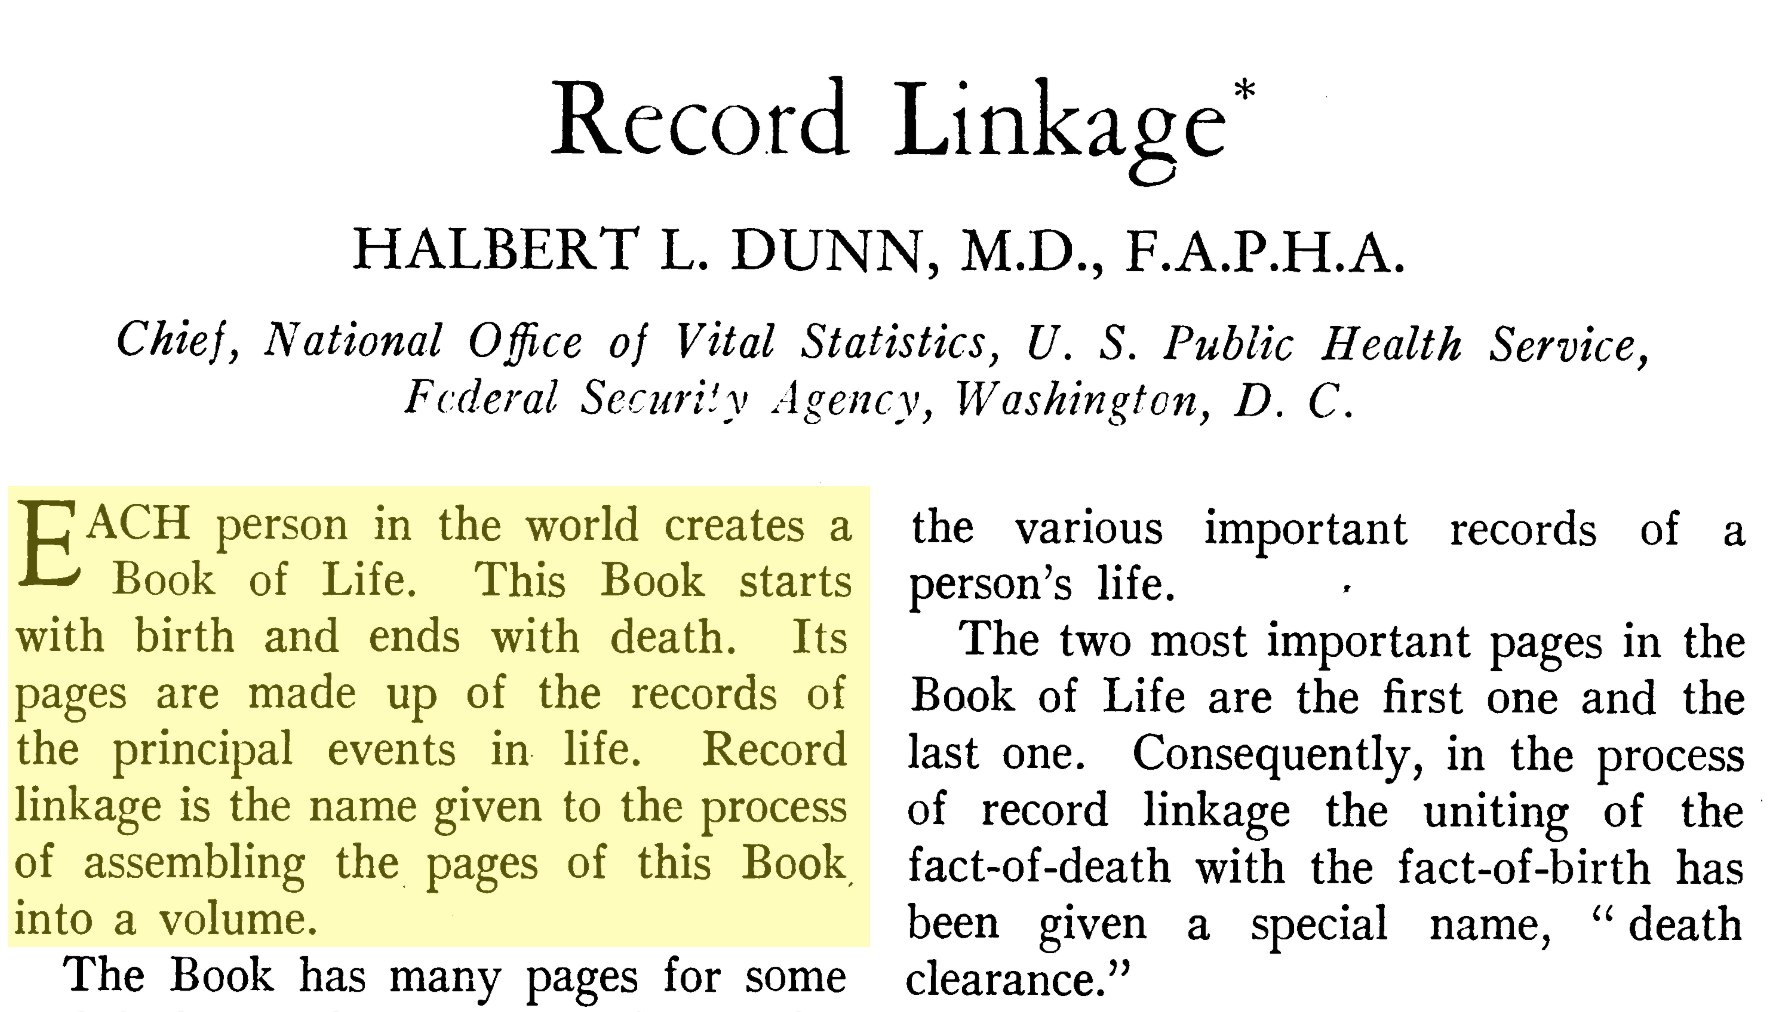
\includegraphics[scale=0.35]{finalFigures/dunn}
%\caption{default}
%\label{default}
\end{center}
\end{figure}


}


\frame{

\begin{figure}[htbp]
\begin{center}
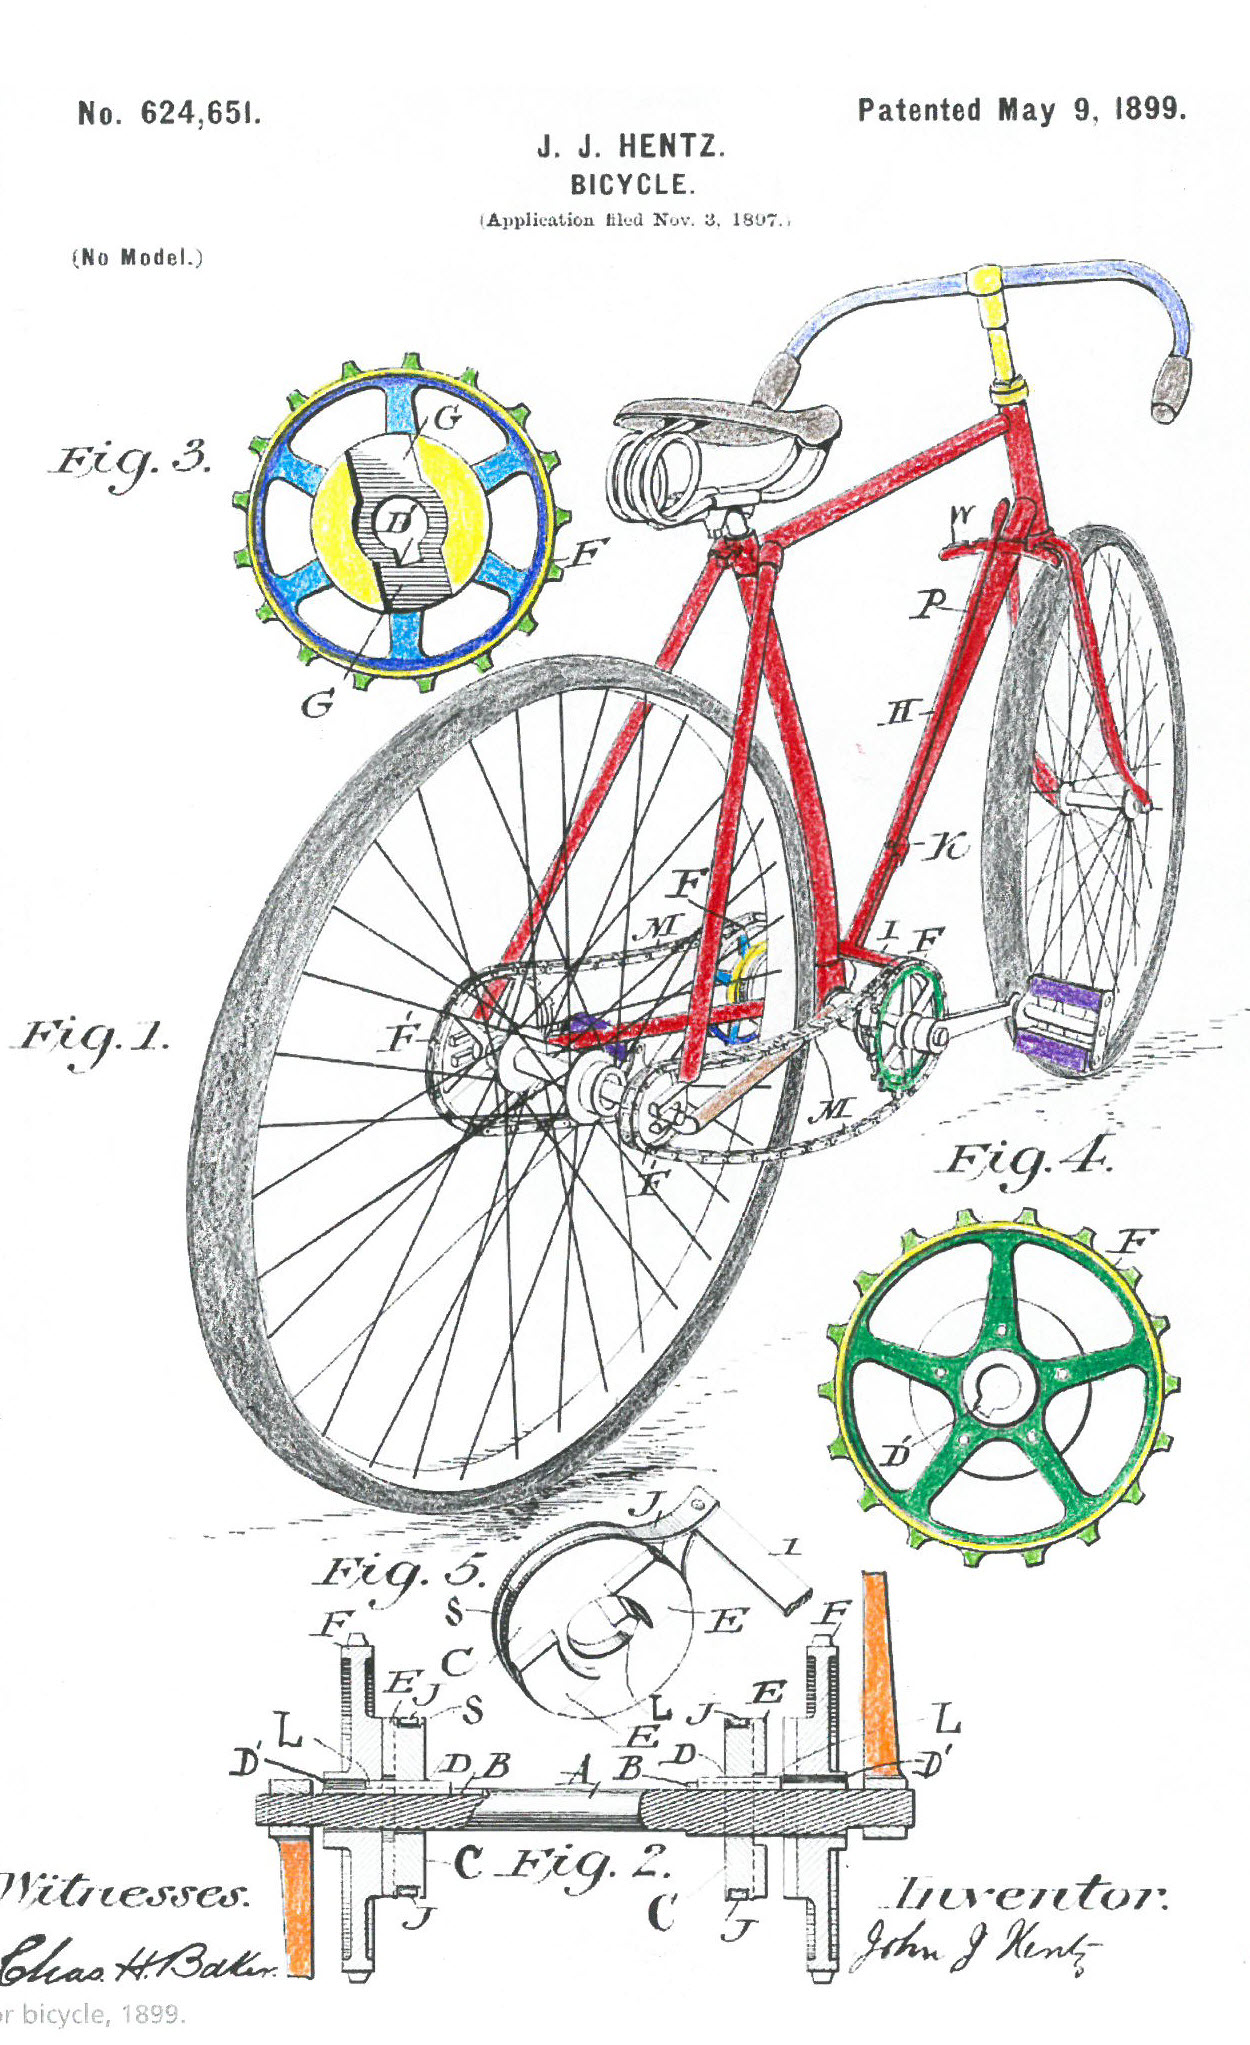
\includegraphics[scale=0.35]{finalFigures/BicyclePatent}
%\caption{default}
%\label{default}
\end{center}
\end{figure}


}


\frame{

\center
\begin{figure}[htbp]
\begin{center}
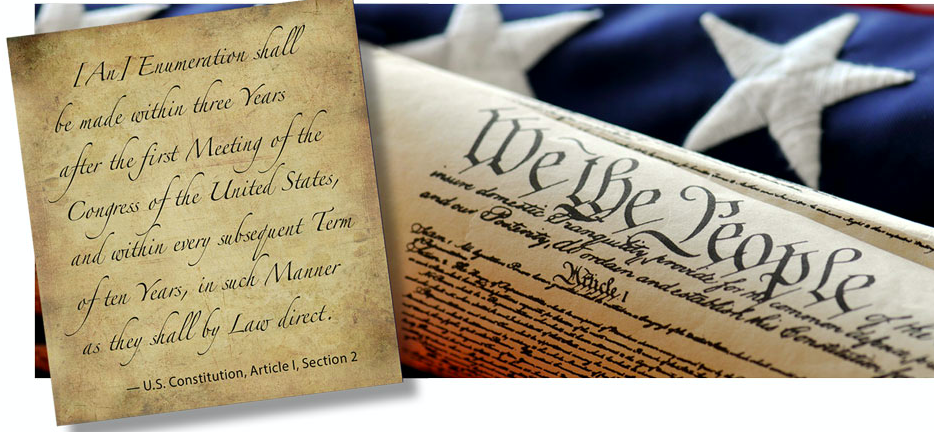
\includegraphics[scale=0.45]{finalFigures/census-hero2}
%\caption{default}
%\label{default}
\end{center}
\end{figure}

%``The actual enumeration shall be made within three Years after the first Meeting of Congress of the United States, and within every subsequent Term of ten Years, in such Manner as they shall by Law direct.""
%
%\vspace*{1em}

%Article I, Section II, U.S. Constitution 

}


\frame{

\begin{figure}[htbp]
\begin{center}
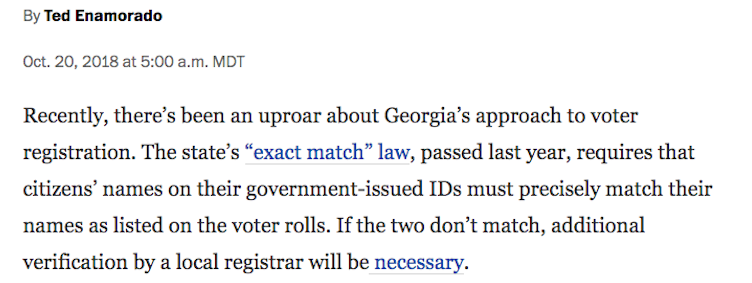
\includegraphics[scale=0.35]{finalFigures/voter-issues-2}
%\caption{default}
%\label{default}
\end{center}
\end{figure}

\pause
\vspace*{1em}

This is an example of a situation where a voter named ``Roberto Juan Hernandez Ruiz" and ``Roberto Ruiz" would be flagged. 

%This law caused voters to be flagged that had four names, such as ``Alexa Olivier Jones Robert" or ``Roberto Juan Hernandez Betancourt."

%%For passports, you can now have 35 characters for first-name, middle-name, and last-name. Not sure about driver's licenses. 

%% For voter registration in GA, you get 40 characters for last name, 30 for first and middle name. 

%% So, this would bias only people with extremely long names. 


}

%\begin{figure}[htbp]
%\begin{center}
%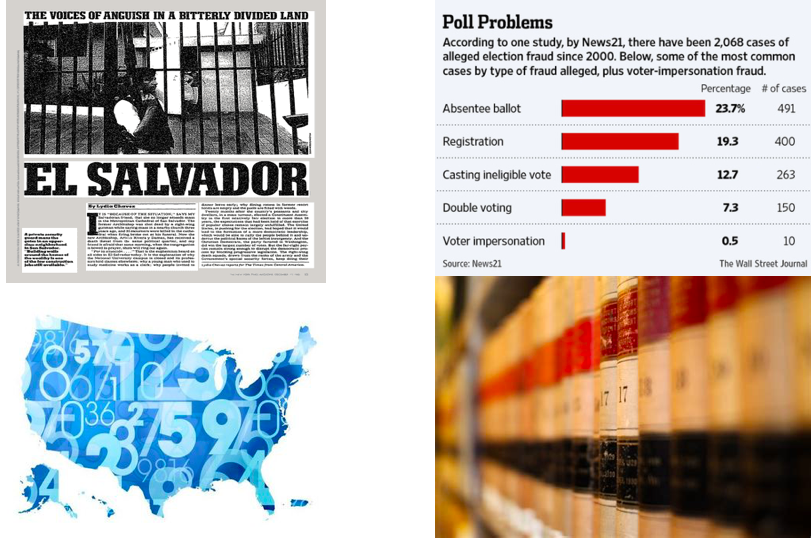
\includegraphics[scale=0.35]{finalFigures/running-examples}
%%\caption{default}
%%\label{default}
%\end{center}
%\end{figure}




%\frame{
%
%\begin{enumerate}
%\item Decennial Census
%\item Documented Identifiable Deaths in El Salvador 
%\item Estimation of Voters in North Carolina 
%\item Inventor and Author Disambiguation 
%\end{enumerate}
%
%}

\frame{
\center
\Large

Terminology

}

%\frame{
%
%\begin{enumerate}
%\item  \textit{Databases} or \textit{files} are collections of \textit{records} which refer to \textit{entities} (such as a person, an object or an event). 
%\item Each record contains information listed under a set of \textit{attributes}, \textit{fields} or \textit{features}, such as the person's age, name, etc. 
%\item An attribute is a \textit{unique identifier} if two records refer to the same entity exactly when the unique identifiers are the same (for example, a birth number).
%\end{enumerate}
%
%}




%\frame{
%
%\begin{enumerate}
%\item \textit{Deduplication} (or duplicate detection) refers to removing duplicate records within one database. 
%\item \textit{Record linkage} refers to merging together multiple databases and removing duplicate entities across the databases, but not within the databases. \item \textit{Entity resolution} refers to simultaneously merging together multiple databases and removing duplicate records across and within databases. \end{enumerate}
%
%}

\frame{
\frametitle{The linkage graph}
\begin{figure}[htbp]
\begin{center}
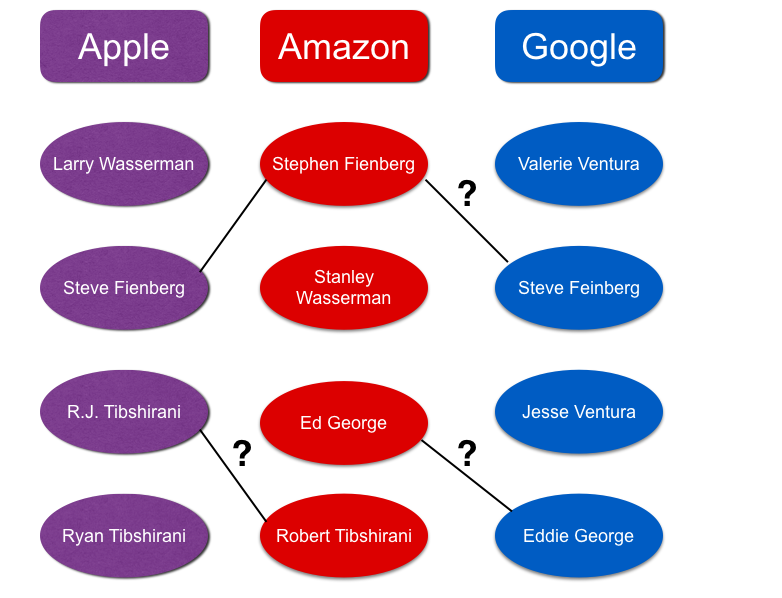
\includegraphics[scale=0.35]{finalFigures/linkage2}
%\caption{default}
%\label{default}
\end{center}
\end{figure}

}

\frame{
\frametitle{The attribute (full name) of Larry Wasserman}
\begin{figure}[htbp]
\begin{center}
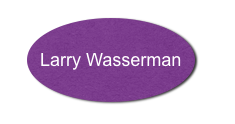
\includegraphics[scale=0.35]{finalFigures/node}
%\caption{default}
%\label{default}
\end{center}
\end{figure}

}

\frame{
\frametitle{The collection of the record of Larry Wasserman}
\begin{figure}[htbp]
\begin{center}

\includegraphics[scale=0.35]{finalFigures/node-feature}
%\caption{default}
%\label{default}
\end{center}
\end{figure}
}

\frame{
\frametitle{De-duplication, Record linkage, and Entity resolution}
\begin{figure}[htbp]
\begin{center}
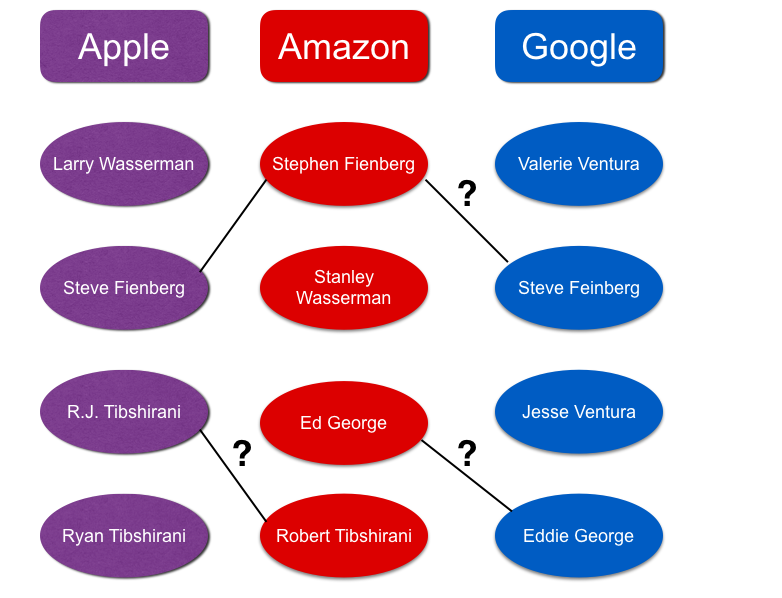
\includegraphics[scale=0.35]{finalFigures/linkage2}
%\caption{default}
%\label{default}
\end{center}
\end{figure}

}

%\frame{
%
%Given multiple records refering to the same entity, \textit{canonicalization} (or data merging and data fusion) is the process constructing a single record which is representative of the whole and which resolves potentially conflicting information. 
%
%
%
%}





\frame{
\center
\Large

Challenges

}

\frame{
\frametitle{Challenges of Entity Resolution}

\begin{figure}[htbp]
\begin{center}
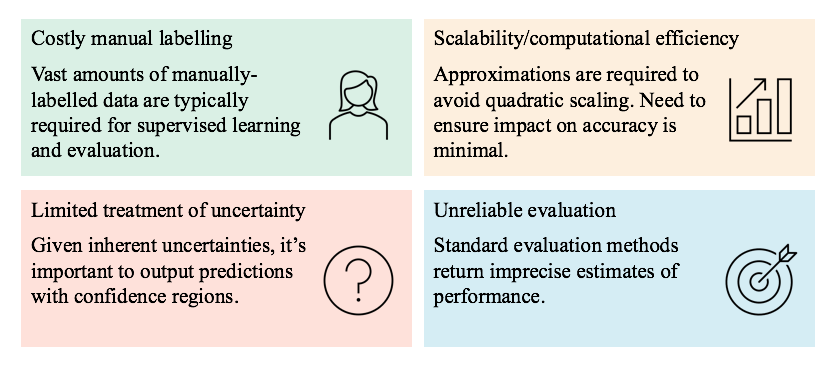
\includegraphics[scale=0.35]{finalFigures/pain-points}
%\caption{default}
%\label{default}
\end{center}
\end{figure}

}

%\frame{
%Entity resolution is difficult because of the need to balance between: 
%
%\begin{enumerate}
%\item efficient methods which scale to large databases
%\item accurate, robust and generalizable methods which make maximal use of all available information, and 
%\item appropriately quantifying and propagating uncertainty coming from all stages of the entity resolution pipeline.
%\end{enumerate}
%
%
%}

\frame{
\center
\Large

Pipeline Approach

}

\frame{
\frametitle{Data Cleaning Pipeline}



%Entity resolution is commonly presented as a pipeline comprising four main stages \citep{christen_data_2012, dong_big_2015}:
%\begin{equation*}
%    \textit{attribute alignment} \rightarrow \textit{blocking} \rightarrow \textit{record linkage} \rightarrow \textit{canonicalization}.
%\end{equation*}
%
%\pause

\begin{figure}[htbp]
\begin{center}
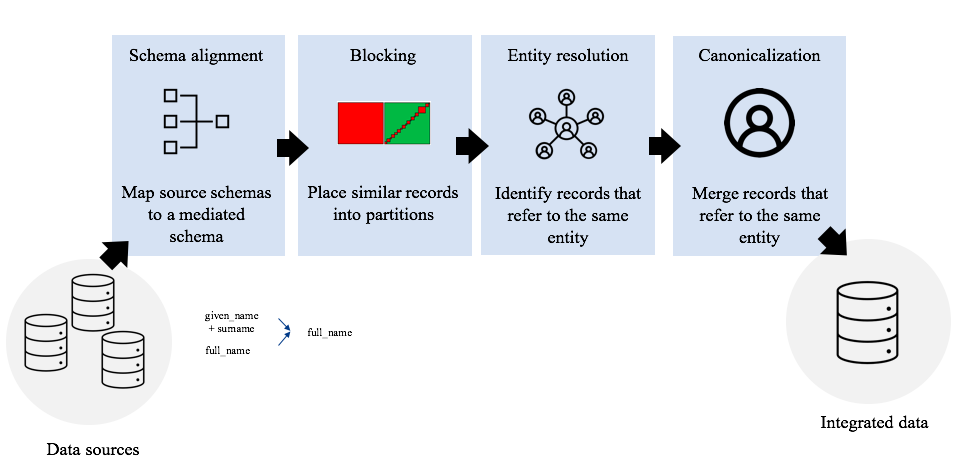
\includegraphics[scale=0.33]{finalFigures/pipeline}
%\caption{default}
%\label{default}
\end{center}
\end{figure}


}





\frame{

\center
\Large
Blocking and Deterministic Record Linkage

}

\frame{

\begin{figure}[htbp]
\begin{center}
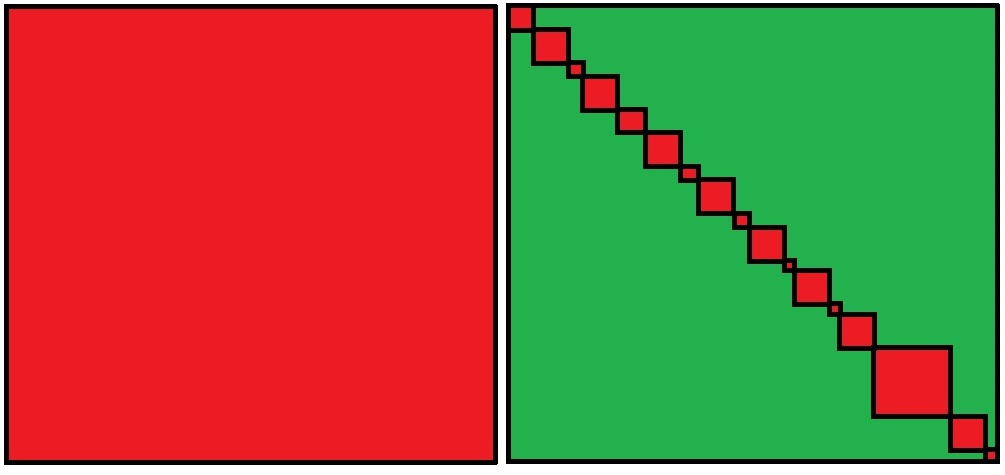
\includegraphics[scale=0.33]{finalFigures/block}
\caption{Left: All to all record comparisons. Right: Similar records placed into the same partition.}
%\label{default}
\end{center}
\end{figure}

Blocking places similar records into a partition. 


}

\frame{

Deterministic record linkage is the most widely used in the literature given that it is
\vspace*{1em}

\begin{enumerate}
\item scalable
\item rules that can easily be put together 
\item and it is easily transferable across disciplines 
\end{enumerate}


}

\frame{
\frametitle{Deterministic Record Linkage}

\begin{enumerate}
\item Exact Matching and Off-by-k Matching
\item Scoring Functions (Edit and Jaro-Winkler distances)
\item Putting simple rules together to form complex rules
\end{enumerate}



}

%\frame{
%\frametitle{Exact Matching}
%
%The simplest form of a deterministic rule is requiring two records to match if they agree on all attributes (date of birth and gender). 
%
%\vspace*{1em} 
%
%\textit{Off by k-matching,} states that two record pairs are a match if they match on all common attributes except $k$, where $k$ is an integer larger 0.
%
%\vspace*{1em} 
%
%This works often works well when all attributes are categorical. 
%
%}
%
%
%\frame{
%\frametitle{Scoring Functions}
%
%Record attributes are often distorted by noise (due to data entry errors, variant spellings, outdated records, etc.).
%
%\vspace*{1em}
%
%One simple way to quantify such differences is via string distance functions, such as the Edit, Jaro, or Jaro-Winkler distances. 
%
%
%}

\frame{
\frametitle{Case Study from the UNTC}

Case study from a human rights conflict in El Salvador from 1980-1992 using data from the United Nations Commission on the Truth (UNTC). 

\scriptsize{
\begin{table}[h]
\begin{center}
\begin{tabular}{ccccccc}
Record & Given name & Family name & Year & Month & Day & Municipality\\\hline
1. &JOSE & FLORES & 1981 & 1 & 29 & A \\
2. &JOSE & FLORES & 1981 & 2 & NA & A \\
3. &JOSE & FLORES & 1981 & 3 & 20 & A \\
4. &JULIAN ANDRES & RAMOS ROJAS & 1986 & 8 & 5 & B\\
5. & JILIAM  & RMAOS  & 1986 & 8 & 5 & B\\
\end{tabular}
\end{center}
\caption{Duplicated records reproduced from Table~1 of Sadinle (2014). Records 1 -- 3 should refer to the same entity. Records 4 -- 5 \emph{might} refer to the same entity. Note that record 5 most likely has OCR errors, where ``RMAOS" should be ``RAMOS." }
\label{table:sv}
\end{table}%
}



}

%\frame{
%
%What happens if we apply exact matching? Does this method do well on Table 1?
%\vspace*{1em}
%
%\pause
%
%What about off-by-k matching? 
%\vspace*{1em}
%
%\pause
%
%What might work better? 
%
%}

\frame{

Sadinle (2014) utilized complex rules for a blocking criteria. 

\vspace*{1em}

Then he applied probabilistic record linkage within each block. 

\vspace*{1em}

Similar rules are used in other human rights applications by Ball (2006); Sadosky, Shrivastava, Price, Steorts (2015); Chen, Shrivastava, Steorts (2018); and in work established by the Human Rights Data Analysis Group (HRDAG). 

\vspace*{1em}
While deterministic rules are recommended for intuition or blocking, they are not recommended in place of probabilistic record linkage. 

\vspace*{1em}
\textbf{Steorts}, Ventura, Sadinle, Fienberg (2014) and Murray (2016) provide reviews on deterministic and probabilistic blocking. 



}

%\frame{
%\frametitle{Rules Using Strings}
%
%Another simple form of a deterministic rule is requiring two records $(r_1, r_2)$ to match if they are similar based upon a defined similarity score 
%$$d(r_1, r_2) > t,$$ were $d$ is any well defined score such as the Edit distance and $t$ is a threshold. 
%
%\vspace*{1em} 
%
%\begin{enumerate}
%\item Example: Consider two attributes ``Rebecca" and ``Rebekah."
%\item Consider the Jaro-Winkler (JW) distance. Let the threshold be 0.70. 
%\item The JW distance between these two names is 0.81, so this rule would state that these two names are the same. 
%\end{enumerate}
%
%}
%
%\frame{
%\frametitle{More Complex Rules}
%
%\begin{enumerate}
%\item More complex rules can be formed using attributes (first name, last name, address, city, others) and decisions can be made. 
%
%\item One a decision has been determined by the rule, it is fixed and cannot be changed (without changing the rule). 
%
%\item Such rules for applications must be carefully considered and tuned. 
%
%\item Given the lack of uncertainty quantification, probabilistic record linkage was developed.
%
%\end{enumerate} 
%
%
%
%
%
%
%
%}
%
%
%\frame{
%\frametitle{More Complex Rules}
%
%\begin{enumerate}
%\item First run blocking pass on dob of birth year. 
%\item Then run a record linkage procedure where we declare all records a match that satisfy the following rule: \end{enumerate} 
%$$\text{distance-last}(r_i,r_j) > 0.7$$ AND  $$\text{distance-first}(r_i,r_j) > 0.7$$
%
%
%}


\frame{

\center
\Large
Probabilistic Record Linkage

}

\begin{frame}
%{Dunn's ``Book of Life''}
    
\begin{center}
    
\includegraphics[width=0.8\linewidth]{finalFigures/Dunn-0}
\end{center}

\textbf{Halbert L. Dunn} (1896-1975):

\begin{itemize}
    \item chief of the National Office of Vital Statistics from 1935-1960.
    \item ``leading figure in establishing a national vital statistics system in the United States''
\end{itemize}

%%The paper ``\textbf{Record Linkage}'':
%%\begin{itemize}
%%    \item adapted from a paper given at the joint conference of the Vital Statistics Council for Canada and for the Dominion Council of Health (Ontario, Canada).
%\end{itemize}
    
\end{frame}

\begin{frame}
%{Dunn's Book of Life}

%\begin{exampleblock}{What this paper does:}

\emph{Record linkage} is the task of assembling together all important pieces of information which refer to the same individual.

%\vspace*{5em}
%Dunn (1946)
\end{frame}

\begin{frame}
%{Dunn's Book of Life}
    \begin{center}
        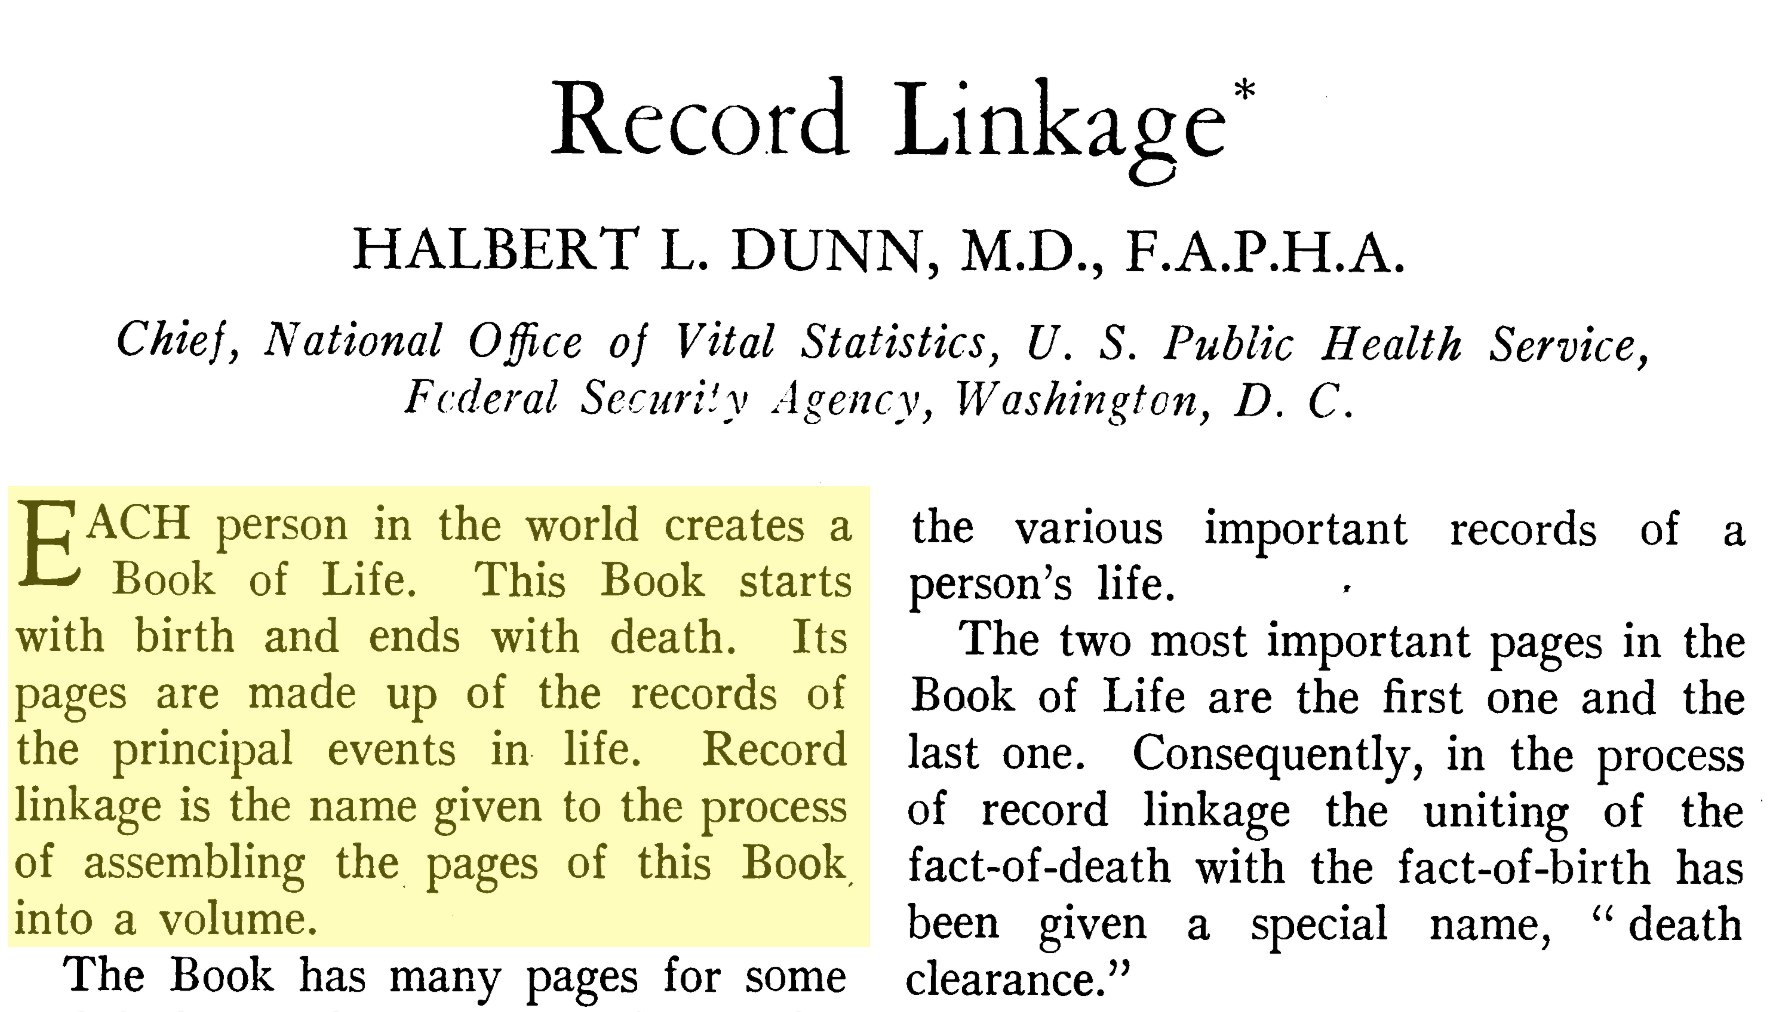
\includegraphics[width=\linewidth]{finalFigures/dunn}
    \end{center}
    

\end{frame}






\begin{frame}
\frametitle{Newcome et al. (1959), Science}
%{Newcombe's computer-based solution}

%Newcombe et al. (1959). Published in \textit{Science}:

\begin{center}
    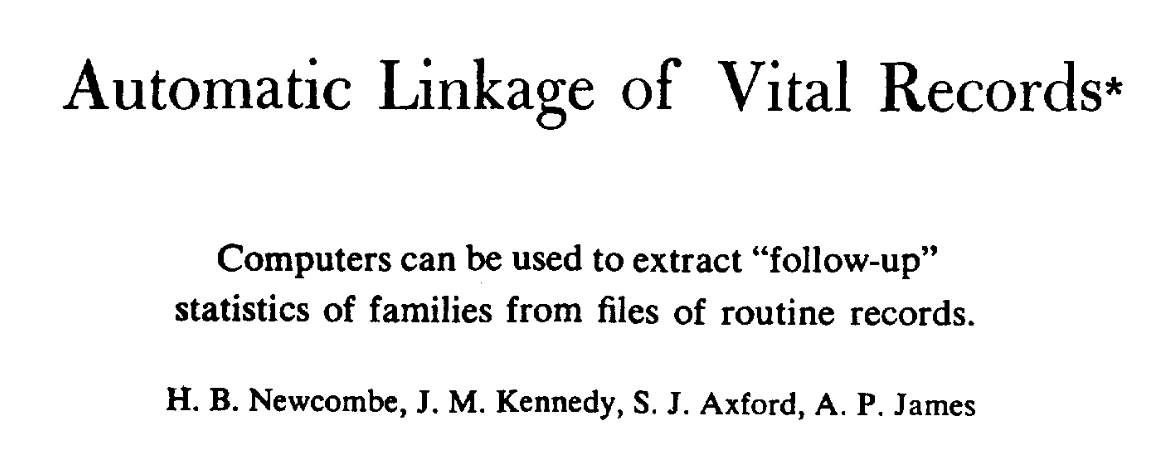
\includegraphics[width=\linewidth]{finalFigures/newcombe}
\end{center}
\end{frame}




\begin{frame}
%{Newcombe's computer-based solution}

Proposed a probabilistic record linkage method and implemented it on the Datatron 205 computer.

\begin{center}
    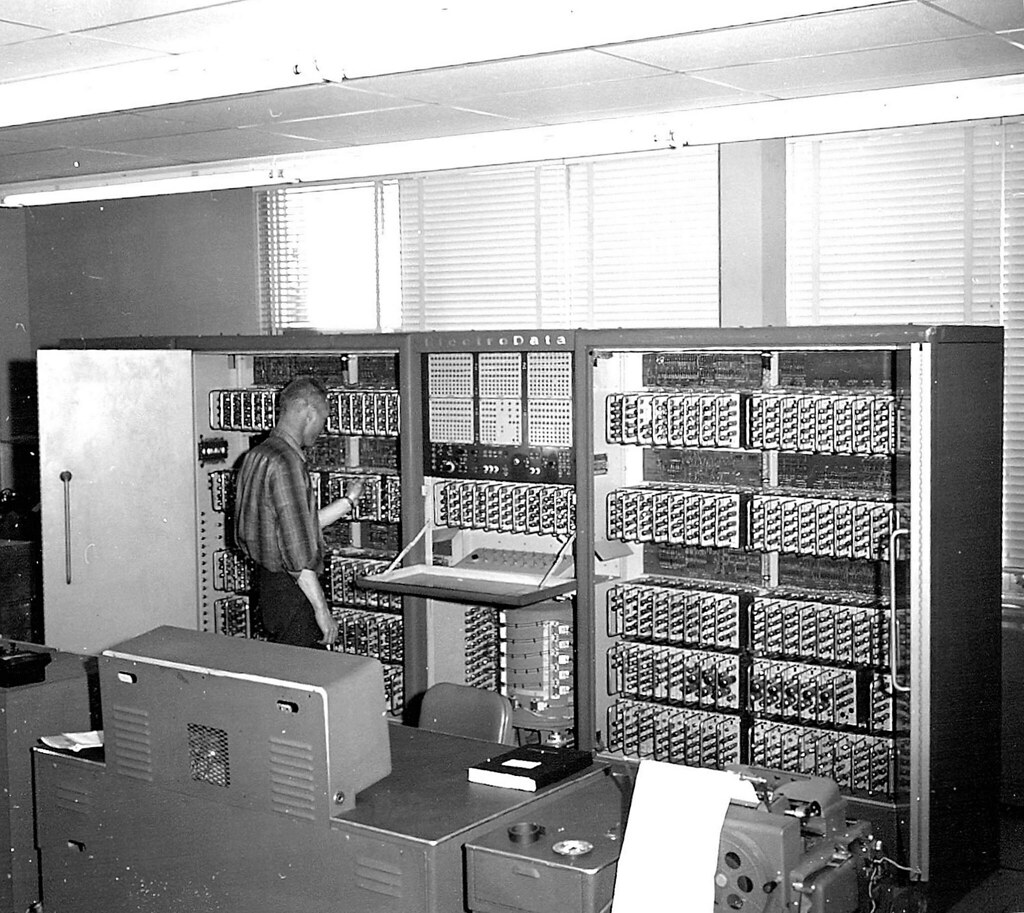
\includegraphics[width=0.6\textwidth]{finalFigures/datatron}
\end{center}

\end{frame}




\begin{frame}
\frametitle{Fellegi and Sunter (1969), JASA}
%{A Theory for Record Linkage}
%Fellegi and Sunter (1969). Published in JASA:
\begin{center}
    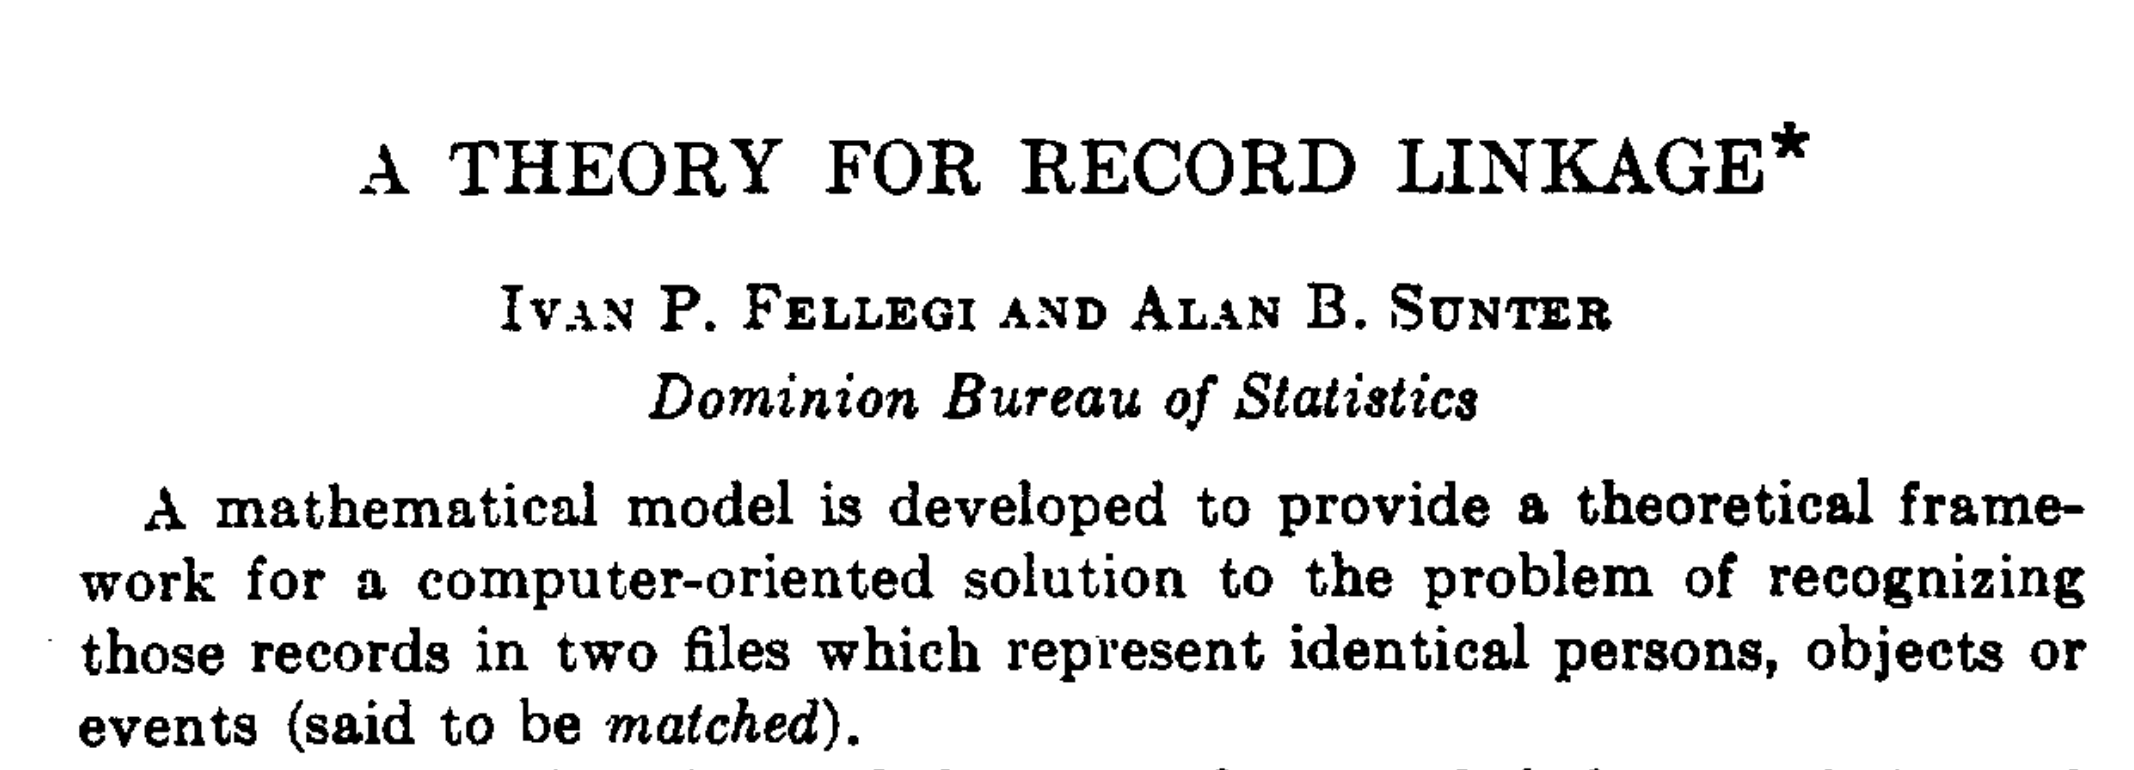
\includegraphics[width=\linewidth]{finalFigures/FS}
\end{center}

\end{frame}




\frame{
\frametitle{Fellegi and Sunter (1969), JASA}

The authors formalized Newcombe et al. (1959) in a decision-theoretic framework. 

\vspace*{1em}

One determines if two records are a match using a likelihood ratio test exceeding a threshold. 


}

\frame{
\frametitle{Fellegi and Sunter (1969), JASA}





There are two methods proposed in this paper. 

\vspace*{1em}


One method is completely unsupervised, and the other is semi-supervised. 

\vspace*{1em}

The semi-supervised methods are used in practice for computational reasons. 

}



\frame{
\frametitle{Fellegi and Sunter (1969), JASA}

Both the methods of Newcombe et al. (1959) and Fellegi and Sunter (1969) have led to extensions that are utilized at statistical agencies in order to update our ``book keeping" regarding an individual's book of life.

\vspace*{1em}

\begin{enumerate}
\item The methods must rely on training data. 
\item There is sensitivity to tuning parameters such as the threshold used. 
\item Both methods on their own do not scale to large data sets. 
\item Transitive closures are not easily satisfied. See Sadinle and Fienberg (2013). 
\end{enumerate}

}


\frame{

\center
\Large
Modern Probabilistic Record Linkage



}



\frame{
\frametitle{fastLink}

The work of Enamorado et al. (2019) extends Fellegi and Sunter (1969) such that 
\begin{enumerate}
\item the authors extend Lahiri and Larsen (2005) to incorporate auxiliary information such as population name frequency and migration rates into the merge procedure to conduct post-merge analyses
\item the authors are able to account for uncertainty of the merge process 
\item the authors use parallelization and efficient data representations such that they can scale to millions of records
\end{enumerate}
\vspace*{1em}

This work has been extended by Enamorado and \textbf{Steorts} (2020) to utilize fastLink as proposal for probabilistic blocking. 

}



\frame{
\frametitle{Bayesian FS Methods}

Sadinle (2014) is a Bayesian Fellegi-Sunter method for de-duplication using a likelihood ratio similar in spirit to Fortini et al. (2001) and Fellegi and Sunter (1969). 

\vspace*{1em}

The author considers a prior on the matching configuration matrix which imposes \textit{transitive closures} --- records are partitioned into groups which are thought to refer to the same entity.

\vspace*{1em}

This allows for uncertainty quantification via the posterior distribution. 

\vspace*{1em}

The author provides corrections and a small labelled set of records for the UNTC data set as well a case study. 

}

\frame{
\frametitle{Bayesian FS Methods (Continued)}

\vspace*{1em} 

Sadinle (2017) extended this work to bipartite record linkage and derived Bayes estimates under a general class of loss functions, providing an alternative to the FS decision rule. 

\vspace*{1em} 

McVeigh et al. (2020) is an extension of Sadinle (2014, 2017) to include probabilistic blocking before the use of Bayesian FS. 

\vspace*{1em} 

The authors greatly improve the speed of the original approach of Sadinle and apply this methodology to a case study on voter registration and historical census records from California. 
 

%Sadinle (2018) proposed a two-stage approach to record linkage and multiple-systems estimation (MSE). 
%
%\vspace*{1em} 
%
%The author first removed duplications from the El Salvador dataset and then utilizes a MSE methodology in order estimate the unknown population size. 
 


}


%\frame{
%\frametitle{Blocking and Bayesian FS}
%
%
%}

\frame{
\frametitle{Semi-supervised and fully supervised methods}

Semi-supervised methods use a relatively small amount of manually classified record pairs, known as labeled pairs, to improve upon unsupervised probabilistic record linkage.

\vspace*{2em} 

Fellegi and Sunter (1969), Belin and Rubin (1995), Nigam et al. (2000), Larsen and Lahiri (2005), Chapelle et al. (2006), Christen et al. (2015), Kejriwal and Miranker (2015), Enamorado et al. (2019).

}

\frame{



Fully supervised methods do not exploit information provided by unlabeled examples; instead they rely on larger amounts of labeled pairs.

\vspace*{1em} 

\begin{enumerate}
\item Training data may come from approximate training sets (using unsupervised ER)
\item Training data may come by manual labelling of data 
\item Training data may come from crowdsourcing extensive manual record linkage efforts. 
\end{enumerate}

\vspace*{1em} 

Approximate training sets: Torvik et al. (2015)\\
\vspace*{1em} 
Crowdsourcing: Sarawagi and Bhamidipaty (2002), Wang et al. (2012), Vesdapunt et al. (2014), Frisoli et al. (2019). \\
\vspace*{1em} 
Manual efforts: Flemming et al. (2007), Christen (2007, 2008, 2014), Li et al. (2014), Ventura et al. (2014, 2015). 

}








\frame{

\center
\Large
Clustering Based Methods 

}


%\frame{
%
%
%
%Clustering as a post-processing step (Similarity graph approaches), Graphical ER (latent entity approaches), Microclustering (make this part very simple).
%
%
%
%}

%\frame{
%
%Clustering as a post-processing step (Similarity graph approaches)
%
%
%}

%\frame{
%
%Graphical ER (latent entity approaches),
%
%SHF14, SHF16, S15, S17, 
%
%}

\frame{
\frametitle{Why graphical Bayesian models?}

%\begin{enumerate}
%\item They tend to be data-efficient
%\item Model encodes constraints and prior beliefs about the generative process
%\item Apply Bayes’ rule to update beliefs about unknown parameters (i.e. coreference relation), conditional on observed data
%\item Distributions represent uncertainty in beliefs
%\end{enumerate}

\begin{center}
    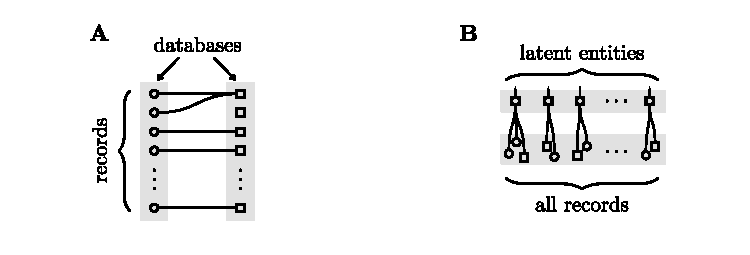
\includegraphics[width=\linewidth]{finalFigures/rl_vs_er}
\end{center}


%\begin{center}
%    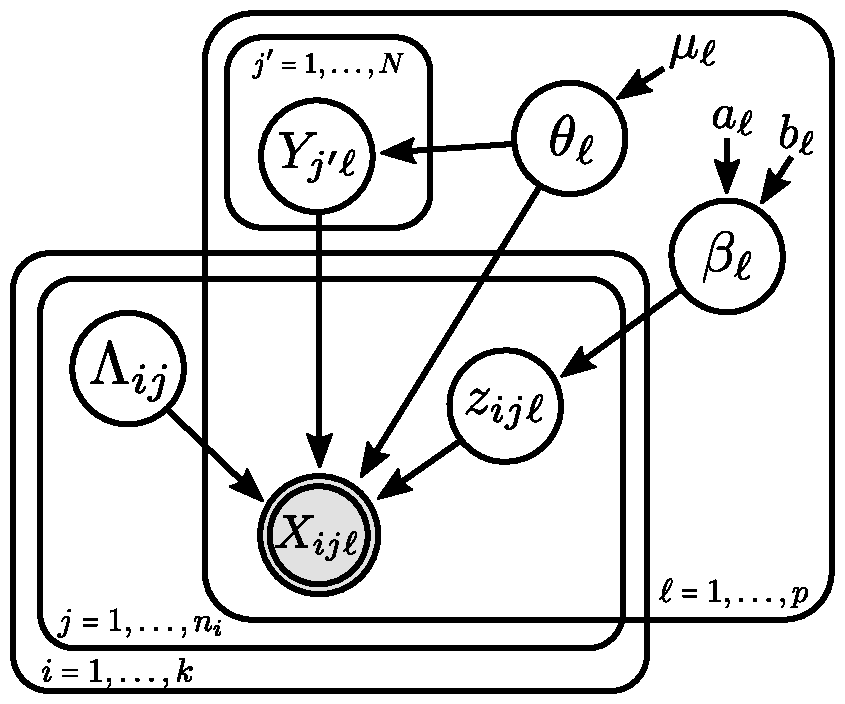
\includegraphics[width=0.5\linewidth]{finalFigures/recordLinkage_graphicalModel}
%\end{center}

\vspace*{1em}

Tancredi and Liseo (2011), Steorts, Hall, Fienberg (2014, 2016), Steorts (2015), Zanella et al. (2016), Steorts, Tancredi, Liseo (2018), Marchant et al. (2020), Tancredi, Steorts, Liseo (2020), Betancourt et. al (2020) 
}

\frame{
\frametitle{distributed graphical entity resolution (\dblink)}

%Marchant et al. (2020) proposed a joint model for blocking and ER

Joint model for blocking and ER:

\begin{enumerate}
%\item Builds of Steorts (2015), adds the joint blocking component 
\item Scales to large databases using partially collapsed Gibbs sampling
\item Distributed inference/parallel inference is possible
\item Many computational speeds ups are proposed 
\item Extensive studies on synthetic and real data sets are given 
\item Open source software is provided in both Apache Spark and R. 
\end{enumerate}

\begin{center}
    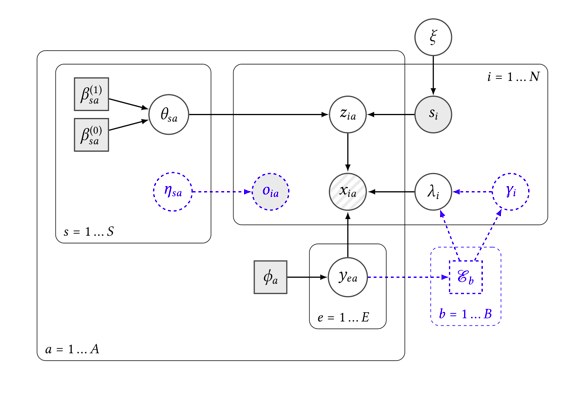
\includegraphics[width=0.5\linewidth]{finalFigures/dblink-model}
\end{center}

Marchant, Kaplan, Elazar, Rubinstein, \textbf{Steorts} (2020), JCGS, In Press. \url{https://arxiv.org/abs/1909.06039}




}

\frame{
\frametitle{\dblink\ applied to synthetic and real data}


\begin{center}
    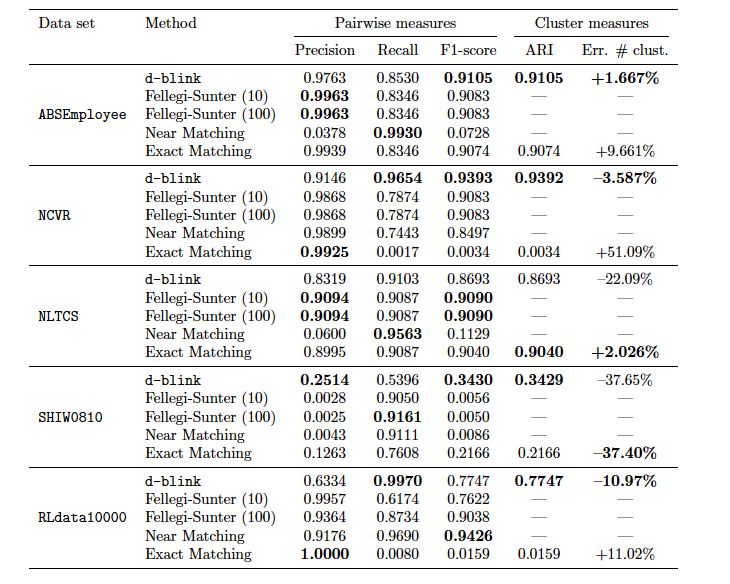
\includegraphics[width=0.9\linewidth]{finalFigures/dblink-exp}
\end{center}

%\begin{center}
%    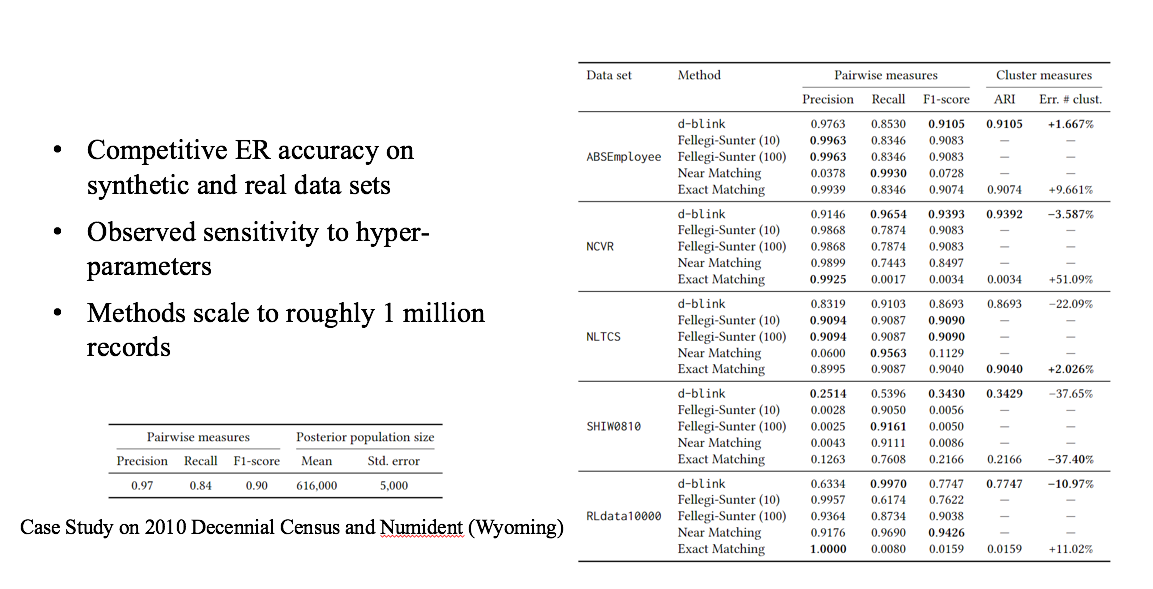
\includegraphics[width=\linewidth]{finalFigures/dblink-results}
%\end{center}

}

\frame{
\frametitle{\dblink\ applied to the 2010 decennial census (Wyoming)}

\begin{enumerate}
\item We consider the 2010 decennial census (Wyoming), which had a raw count of 
563,626. 
\item We merge the 2010 decennial census with administrative records from the 
Social Security Administration's Numerical Identification System (Numident). 
\item We have partial ground truth via social security numbers. 
\item Attributes: first and last name, gender, dob, and zip code. 
\end{enumerate}


\begin{center}
    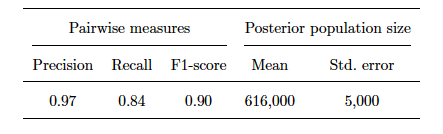
\includegraphics[width=0.9\linewidth]{finalFigures/census-exp}
\end{center}

%\begin{center}
%    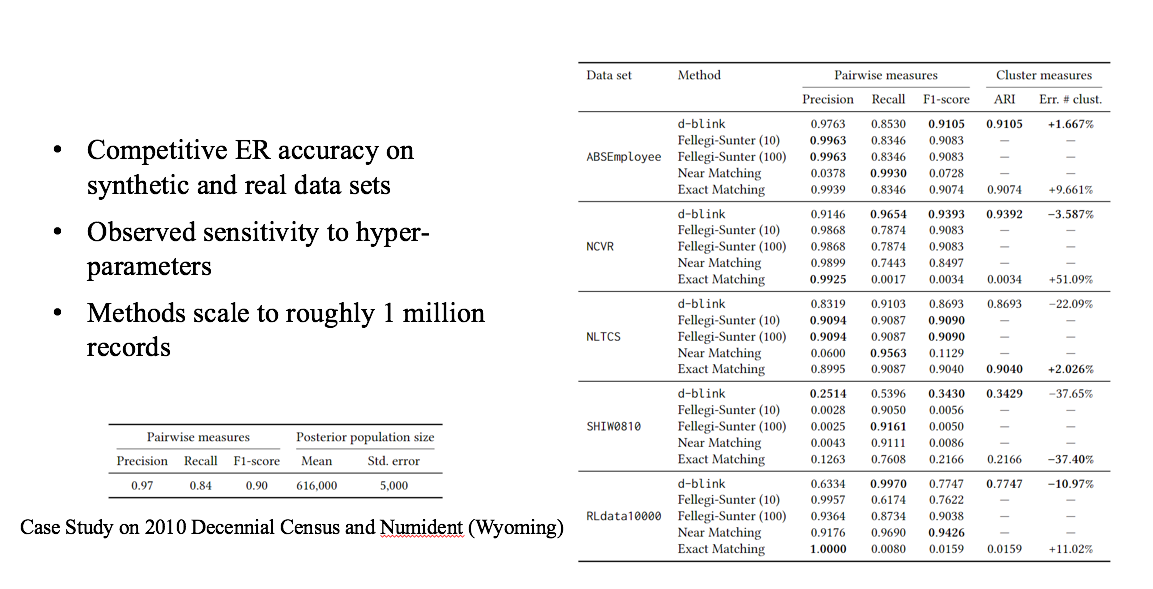
\includegraphics[width=\linewidth]{finalFigures/dblink-results}
%\end{center}

}

%\frame{
%
%Graphical entity resolution led to the realization that as number of records grows (data points), the growth of the size of the clusters grows sub-linearly (and not linearly). 
%
%
%
%}

\frame{
\frametitle{Classical clustering}

\emph{Many clustering tasks require models that assume cluster sizes grow
linearly with the size of the data set.}

\pause
\vskip 1em

Classic examples are the Dirichlet process (DP) and the Chinese Restaurant Process (CRP).
\pause
\vskip 1em
More generally, we think of all infinite mixture models (Pitmor-Yor Process (PYP) and the Kingman Paintbox). 


\begin{figure}[htbp]
\begin{center}
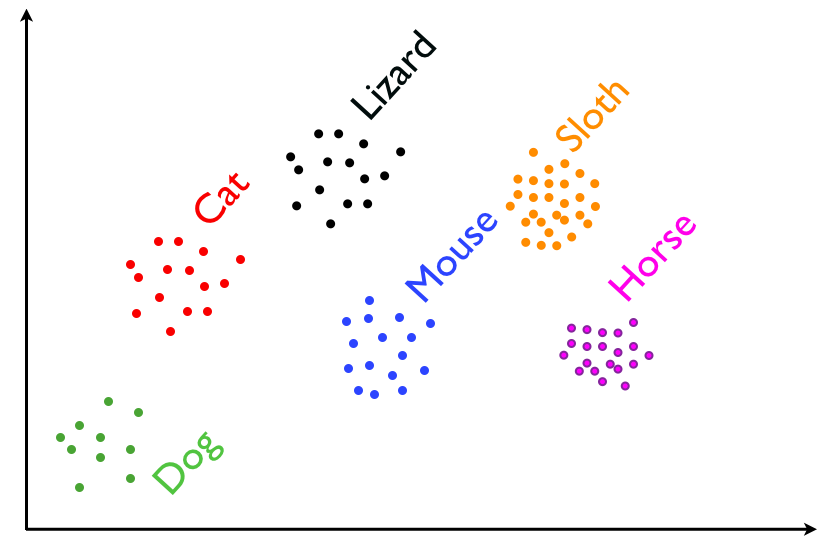
\includegraphics[width=0.6\textwidth]{figures/classicClusters}
\label{default}
\end{center}
\end{figure}

}


\frame{
\frametitle{Flexible Models for Microclustering}

How do we handle data where:
\begin{itemize}
\item We care about the exchangeability of the data points?
\item But as the number of data points grows, the size of each cluster is negligible?
\end{itemize}


}

\frame{
\frametitle{Microclustering}



A sequence of random partitions $(C_N
: N=1, 2, \ldots)$ exhibits the \emph{microclustering property} if $M_N$ is
$o_p(N)$, where $M_N$ is the size of the largest cluster in
$C_N$. 
%Equivalently, $M_N \,/\, N \rightarrow 0$ in probability as $N
%\rightarrow \infty$.

\pause
\vskip 1em
A clustering model exhibits the microclustering property if $(C_N
: N=1, 2, \ldots)$  implied by that model satisfies the above definition.

\vskip 1em

Zanella et al. (2016), Steorts et. al (2017), Johndrow et. al (2018), Betancourt, Zanella, Steorts (2020), Tancredi, Steorts, Liseo (2020).
}





%\frame{
%\frametitle{Consider an example}
%
%\begin{figure}[htbp]
%\begin{center}
%\includegraphics[width=\textwidth]{donors_real.eps}
%%\includegraphics[width=0.5\textwidth]{donors_synthetic.eps}
%\label{default}
%\end{center}
%\end{figure}
%}
%
%
%\frame{
%\begin{figure}[htbp]
%\begin{center}
%%\includegraphics[width=0.5\textwidth]{donors_real.eps}
%\includegraphics[width=\textwidth]{donors_synthetic.eps}
%\label{default}
%\end{center}
%\end{figure}
%}






%\frame{
%\frametitle{Bayesian nonparametric mixture models}
%To cluster $N$ data points $x_1, \ldots, x_N$ using a partition-based
%Bayesian clustering model, one first places a prior over partitions of
%$[N] = \{ 1, \ldots, N \}$.
%\vspace*{1em}
%
%\pause
%$C_N$ is
%implicitly represented by a set of cluster assignments $z_1, \ldots,
%z_N$. 
%}
%
%\frame{
%\frametitle{New Approach}
%
%\begin{itemize}
%\item Propose a model that satisfies the microclustering property.
%\item Seek flexible and robust models. 
%\item New sampling algorithm. 
%\item Results on real data from medicine, official statistics, and the Syrian conflict. 
%\end{itemize}
%
%Zanella et al. (2016), Betancourt et al. (2020).
%
%}




\frame{

\center
\Large
Life After Entity Resolution: \\Canonicalization and Downstream Tasks

}

\frame{

\center
\Large

Canonicalization, merging, or data fusion is the task of merging groups of records that have been classified as matches into one record that represents the true entity. 





%Canonicalization, MSE, Downstream Tasks (Joint Models and Two-Stage Models).
%
%Culotta07+, Kaplan20+, STL18, TSL20, TRS20, Sadinle18, Others?



}

\frame{

\begin{enumerate}
\item The earliest proposals of canonicalization were deterministic, rule-based methods, which were application specific and fast to implement (Cohen and Sagiv, 2005).
\item The existing literature assumes training is available in order to select the canonical record, and authors have proposed optimization and semi-supervised methods to find the most representative record. 
\item Motivated by the NCSBE voters data set, Kaplan et al. (2020) provide a unique identifier for voter registration in a principled and reproducible manner. 
\item For a full review of data fusion techniques, we refer to Bleiholder
and Naumann, 2009. 
\end{enumerate}

Christen (2012), Culotta et al (2007), Bleiholder
and Naumann (2009). 
}

\frame{

Turning to joint or single-stage modeling approaches to entity resolution and the downstream task, these have been limited to linking two databases and do not easily generalize beyond this framework. 

\vspace*{1em}

Recent applications to human rights data have been done by Sadinle (2018) and Tancredi, Steorts, and Liseo (2020) involving population sized estimation (multiple systems estimation). 

\vspace*{1em}

Single-stage, joint models, and canonicalization tasks cover a vast body of literature. For a more thorough review, be on the look out for a review paper by Binette and Steorts (2020) on entity resolution. 

}


\frame{
\frametitle{Open Research Problems and Discussion Questions}

\begin{enumerate}
\item How should one do fair comparisons and evaluations? 
\item How should one create training data sets? 
\item How should one find publicly available benchmark data sets and which ones should be used? 
\item Should we be aware that entity resolution can be used for massive data collection efforts and evasion of privacy? What can we do as a field regarding this? 
\item What privacy guarantees are offered for record linkage? 
\item What ethical considerations do I have when working with private data that is sensitive, such as the data that HRDAG provides? 
\item What resources are available to me if I want to know more about the field of record linkage? 
\end{enumerate}

}


\frame{

\center
\Large
Questions?\\
beka@stat.duke.edu\\
Webpage: \url{resteorts.github.io} \\ 
Software: \url{https://github.com/orgs/cleanzr/}\\
Paper: \url{https://arxiv.org/abs/2008.04443}


}

\clearpage
\newpage
\bibliographystyle{jasa}
\bibliography{er-review}

\newpage
\appendix

\frame{
\frametitle{CRP Behavoir for N increasing and $\alpha$ fixed}

\begin{figure}[htbp]
\begin{center}
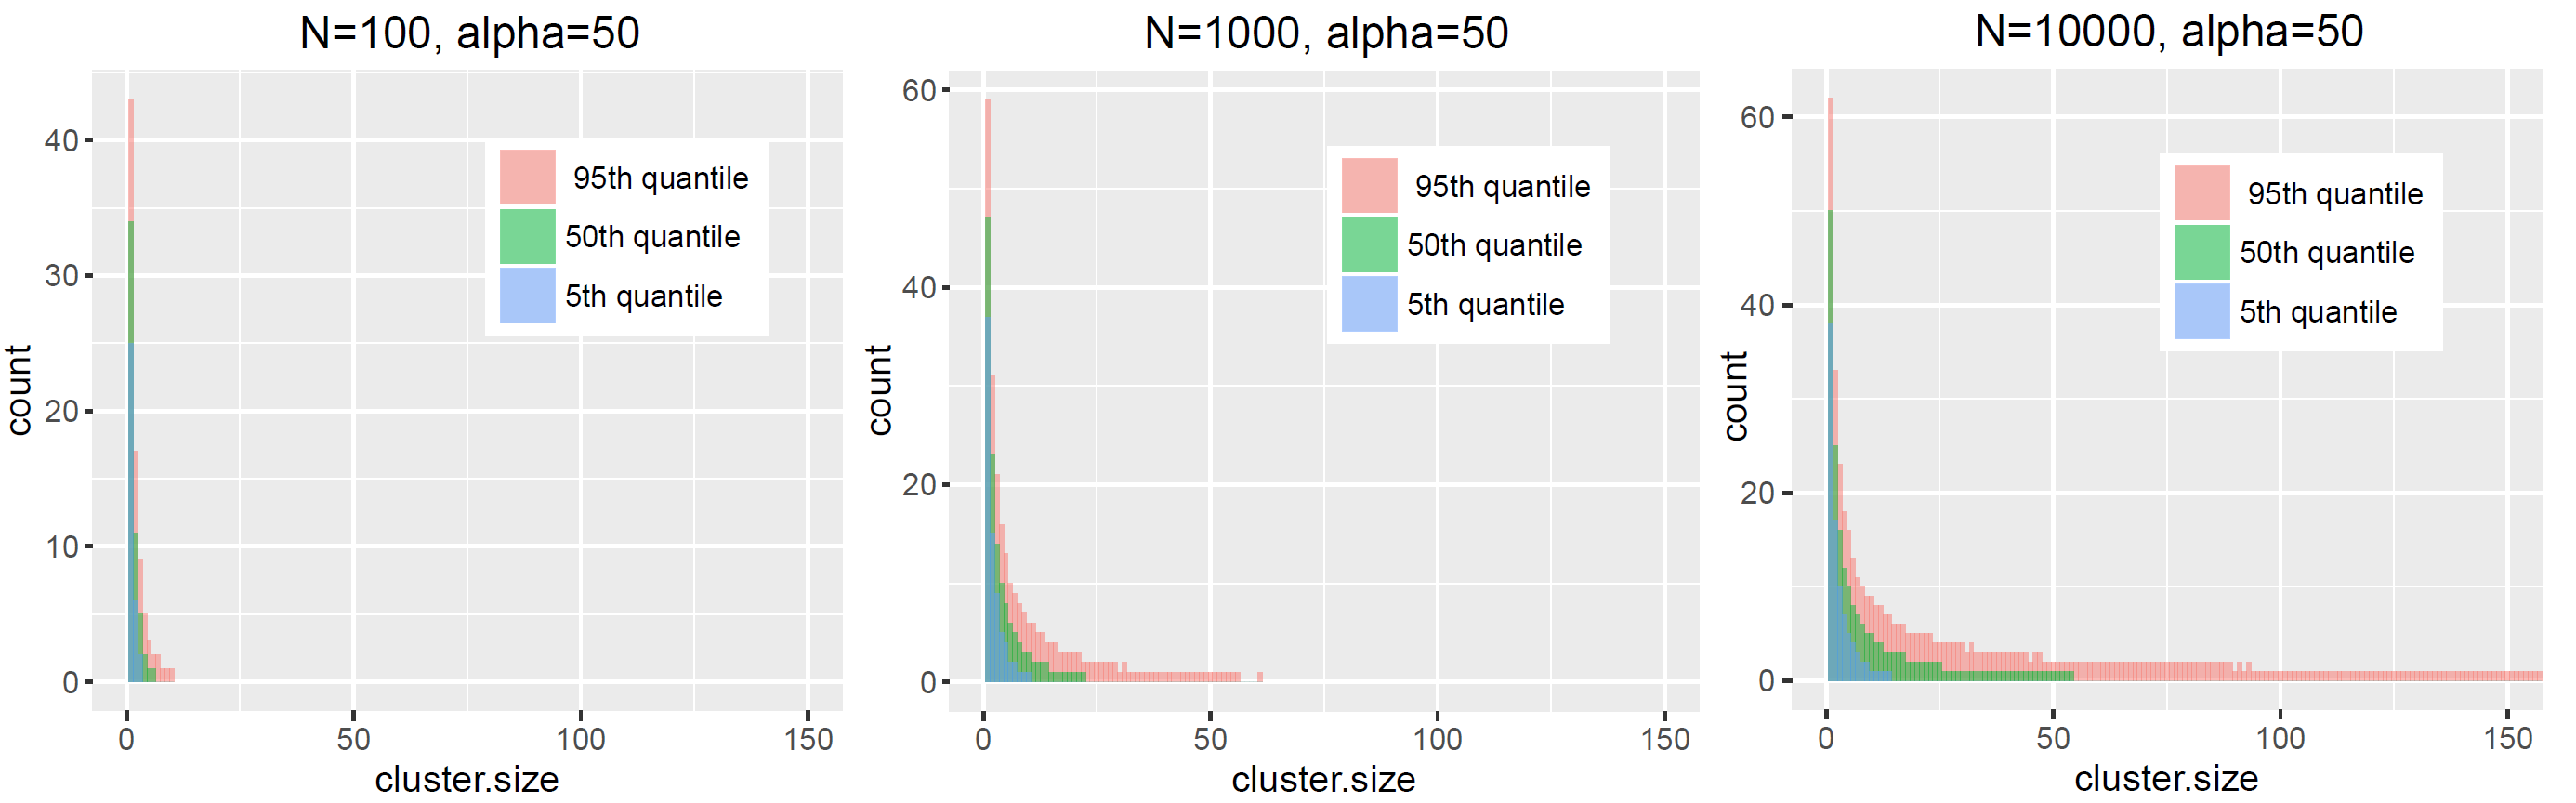
\includegraphics[width=\textwidth]{figures/CRP_N_increasingand_alpha_fixed}
%\includegraphics[width=0.5\textwidth]{donors_synthetic.eps}
\label{eqn:infinite}
\end{center}
\end{figure}

As $N$ increases the size of the clusters increases as $O(N) \implies$
Not appropriate for microclustering. 

}

\frame{
\frametitle{CRP Behavoir for N and $\alpha$ jointly increasing}

\begin{figure}[htbp]
\begin{center}
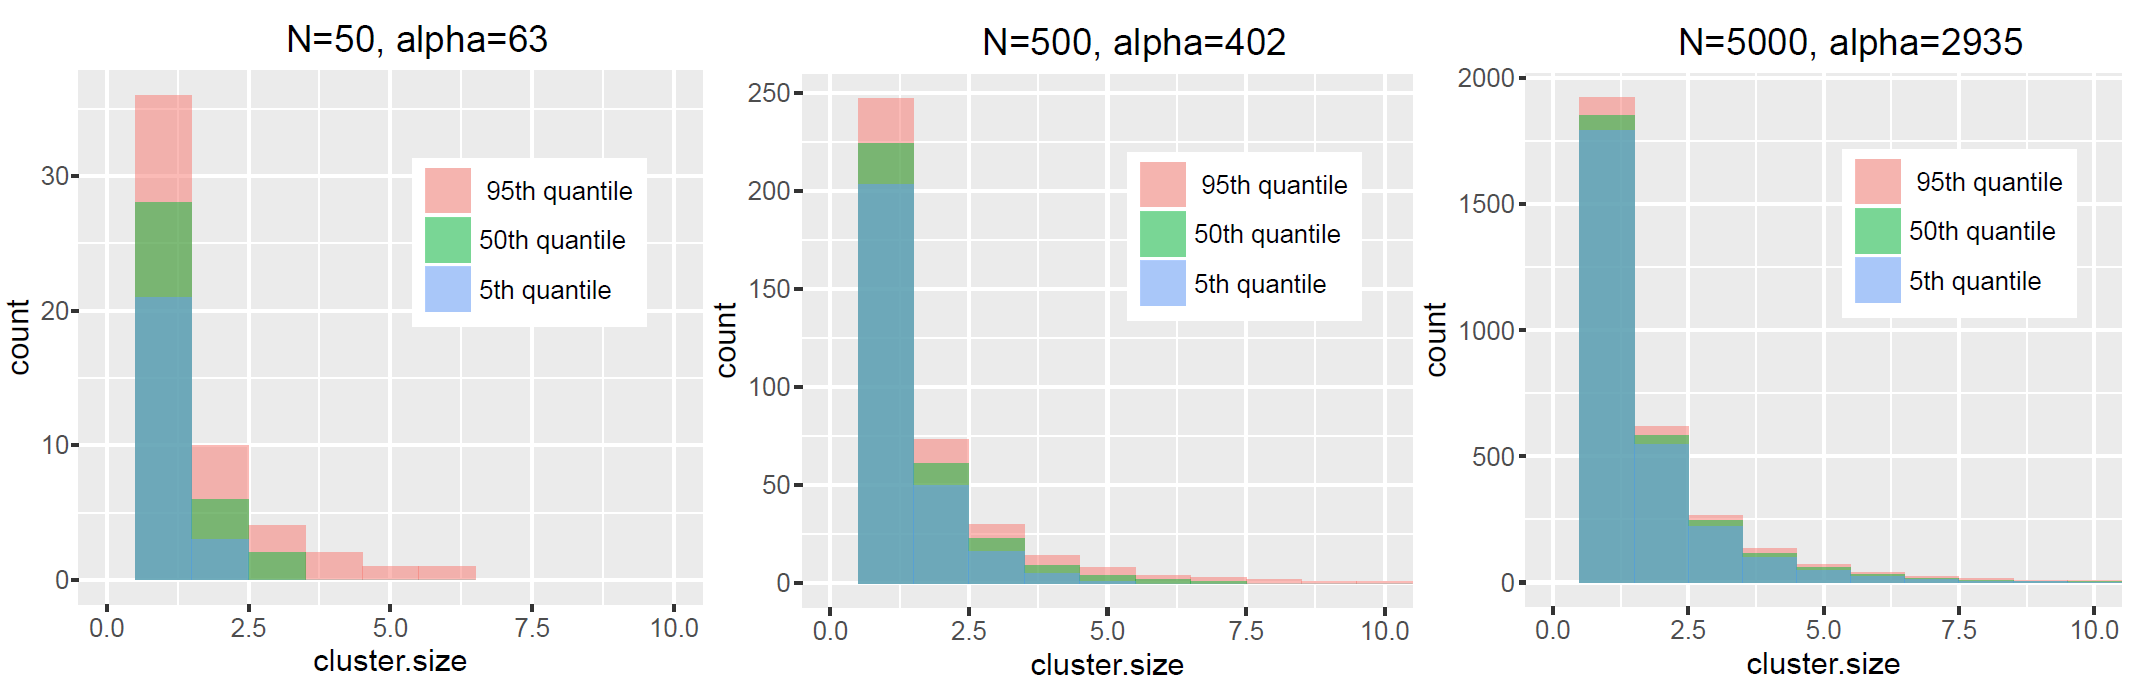
\includegraphics[width=\textwidth]{figures/CRP_N_and_alpha_increasing}
%\includegraphics[width=0.5\textwidth]{donors_synthetic.eps}
\label{eqn:infinite}
\end{center}
\end{figure}

Can obtain microclustering property by increasing $\alpha$ with $N$ but the 
resulting model becomes less flexible.
\vskip 1em

The model collapses onto a one parameter family distribution for the cluster sizes. 

\vskip 1em

This behavior motivates models that naturally incorporate the microclustering property.
}


\end{document}